
\begin{table}[htb]
    \renewcommand{\arraystretch}{1.5}
    \begin{tabular*}{\textwidth}{|>{\columncolor{red!40}}p{3cm}|p{17.3cm}|}
    \textbf{\large Finding} & \textbf{\large Root access via authorized keys entry of user bluey}\section*{}\addcontentsline{toc}{section}{Finding 11 - Root access via authorized keys entry of user bluey}\label{chap:Insecure}
    \\
    Risk& Critical\\
    Category& Privilege Escalation, Misconfiguration\\
    Impact& An attacker with access to user bluey can gain root access\\\\
    Description& The authorized\_keys file in the root directory has an entry.
    \begin{lstlisting}[language=bash]
plunder [~/.ssh]: cat authorized_keys
ssh-ed25519 AAAAC3NzaC1lZDI1NTE5AAAAIMO EhQP4e3BVrq0R9nPQz folf9349W/UDXSAbQIj6RDM joe@reliant
ssh-ed25519 AAAAC3NzaC1lZDI1NTE5AAAAINV2RROAIF7+9Cm7U2PWVTmJx0hjvTQeYF04L07 Et1qk bluey@plunder
    \end{lstlisting}
    Given this information it is feasible to obtain root access by logging into the root account via ssh without using password.
    \newline
    \newline
    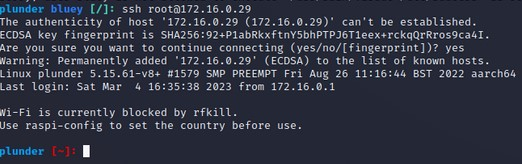
\includegraphics{root_login.jpg}
    
	\\\\\\
    Recommendation& To address this vulnerability, it is recommended to remove the public key of the bluey user from the authorized\_keys file of the root user. Additionally, it is generally advised not to permit user access to the Device Under Test (DUT) via SSH as the root user.\\
    \\\\\\\\\\\\\\\\\\\\\\\\\\\\\\\\\\
    \end{tabular*}
    \end{table}